\documentclass[twoside]{book}

% Packages required by doxygen
\usepackage{fixltx2e}
\usepackage{calc}
\usepackage{doxygen}
\usepackage[export]{adjustbox} % also loads graphicx
\usepackage{graphicx}
\usepackage[utf8]{inputenc}
\usepackage{makeidx}
\usepackage{multicol}
\usepackage{multirow}
\PassOptionsToPackage{warn}{textcomp}
\usepackage{textcomp}
\usepackage[nointegrals]{wasysym}
\usepackage[table]{xcolor}

% Font selection
\usepackage[T1]{fontenc}
\usepackage[scaled=.90]{helvet}
\usepackage{courier}
\usepackage{amssymb}
\usepackage{sectsty}
\renewcommand{\familydefault}{\sfdefault}
\allsectionsfont{%
  \fontseries{bc}\selectfont%
  \color{darkgray}%
}
\renewcommand{\DoxyLabelFont}{%
  \fontseries{bc}\selectfont%
  \color{darkgray}%
}
\newcommand{\+}{\discretionary{\mbox{\scriptsize$\hookleftarrow$}}{}{}}

% Page & text layout
\usepackage{geometry}
\geometry{%
  a4paper,%
  top=2.5cm,%
  bottom=2.5cm,%
  left=2.5cm,%
  right=2.5cm%
}
\tolerance=750
\hfuzz=15pt
\hbadness=750
\setlength{\emergencystretch}{15pt}
\setlength{\parindent}{0cm}
\setlength{\parskip}{3ex plus 2ex minus 2ex}
\makeatletter
\renewcommand{\paragraph}{%
  \@startsection{paragraph}{4}{0ex}{-1.0ex}{1.0ex}{%
    \normalfont\normalsize\bfseries\SS@parafont%
  }%
}
\renewcommand{\subparagraph}{%
  \@startsection{subparagraph}{5}{0ex}{-1.0ex}{1.0ex}{%
    \normalfont\normalsize\bfseries\SS@subparafont%
  }%
}
\makeatother

% Headers & footers
\usepackage{fancyhdr}
\pagestyle{fancyplain}
\fancyhead[LE]{\fancyplain{}{\bfseries\thepage}}
\fancyhead[CE]{\fancyplain{}{}}
\fancyhead[RE]{\fancyplain{}{\bfseries\leftmark}}
\fancyhead[LO]{\fancyplain{}{\bfseries\rightmark}}
\fancyhead[CO]{\fancyplain{}{}}
\fancyhead[RO]{\fancyplain{}{\bfseries\thepage}}
\fancyfoot[LE]{\fancyplain{}{}}
\fancyfoot[CE]{\fancyplain{}{}}
\fancyfoot[RE]{\fancyplain{}{\bfseries\scriptsize Generated by Doxygen }}
\fancyfoot[LO]{\fancyplain{}{\bfseries\scriptsize Generated by Doxygen }}
\fancyfoot[CO]{\fancyplain{}{}}
\fancyfoot[RO]{\fancyplain{}{}}
\renewcommand{\footrulewidth}{0.4pt}
\renewcommand{\chaptermark}[1]{%
  \markboth{#1}{}%
}
\renewcommand{\sectionmark}[1]{%
  \markright{\thesection\ #1}%
}

% Indices & bibliography
\usepackage{natbib}
\usepackage[titles]{tocloft}
\setcounter{tocdepth}{3}
\setcounter{secnumdepth}{5}
\makeindex

% Hyperlinks (required, but should be loaded last)
\usepackage{ifpdf}
\ifpdf
  \usepackage[pdftex,pagebackref=true]{hyperref}
\else
  \usepackage[ps2pdf,pagebackref=true]{hyperref}
\fi
\hypersetup{%
  colorlinks=true,%
  linkcolor=blue,%
  citecolor=blue,%
  unicode%
}

% Custom commands
\newcommand{\clearemptydoublepage}{%
  \newpage{\pagestyle{empty}\cleardoublepage}%
}

\usepackage{caption}
\captionsetup{labelsep=space,justification=centering,font={bf},singlelinecheck=off,skip=4pt,position=top}

%===== C O N T E N T S =====

\begin{document}

% Titlepage & ToC
\hypersetup{pageanchor=false,
             bookmarksnumbered=true,
             pdfencoding=unicode
            }
\pagenumbering{alph}
\begin{titlepage}
\vspace*{7cm}
\begin{center}%
{\Large A Stressful Machine }\\
\vspace*{1cm}
{\large Generated by Doxygen 1.8.13}\\
\end{center}
\end{titlepage}
\clearemptydoublepage
\pagenumbering{roman}
\tableofcontents
\clearemptydoublepage
\pagenumbering{arabic}
\hypersetup{pageanchor=true}

%--- Begin generated contents ---
\chapter{Hierarchical Index}
\section{Class Hierarchy}
This inheritance list is sorted roughly, but not completely, alphabetically\+:\begin{DoxyCompactList}
\item \contentsline{section}{Game\+Level}{\pageref{classGameLevel}}{}
\item \contentsline{section}{Game\+Sequence}{\pageref{classGameSequence}}{}
\item \contentsline{section}{Virtual\+Machine}{\pageref{classVirtualMachine}}{}
\begin{DoxyCompactList}
\item \contentsline{section}{Virtual\+Machine\+Procedure}{\pageref{classVirtualMachineProcedure}}{}
\end{DoxyCompactList}
\end{DoxyCompactList}

\chapter{Class Index}
\section{Class List}
Here are the classes, structs, unions and interfaces with brief descriptions\+:\begin{DoxyCompactList}
\item\contentsline{section}{\hyperlink{classGameLevel}{Game\+Level} }{\pageref{classGameLevel}}{}
\item\contentsline{section}{\hyperlink{classGameSequence}{Game\+Sequence} }{\pageref{classGameSequence}}{}
\item\contentsline{section}{\hyperlink{classVirtualMachine}{Virtual\+Machine} }{\pageref{classVirtualMachine}}{}
\item\contentsline{section}{\hyperlink{classVirtualMachineProcedure}{Virtual\+Machine\+Procedure} }{\pageref{classVirtualMachineProcedure}}{}
\end{DoxyCompactList}

\chapter{Class Documentation}
\hypertarget{classGameLevel}{}\section{Game\+Level Class Reference}
\label{classGameLevel}\index{Game\+Level@{Game\+Level}}


{\ttfamily \#include $<$Game\+Level.\+h$>$}

\subsection*{Public Member Functions}
\begin{DoxyCompactItemize}
\item 
\mbox{\Hypertarget{classGameLevel_ac990c08a5a5b4956537f88d4fdec23eb}\label{classGameLevel_ac990c08a5a5b4956537f88d4fdec23eb}} 
{\bfseries Game\+Level} (const string \&level\+\_\+name)
\item 
\mbox{\Hypertarget{classGameLevel_a3bfcb4fcadf0eb8918f7b9e956d29d68}\label{classGameLevel_a3bfcb4fcadf0eb8918f7b9e956d29d68}} 
void {\bfseries play} ()
\end{DoxyCompactItemize}


\subsection{Detailed Description}
This class enable the player to complete a level. 

The documentation for this class was generated from the following files\+:\begin{DoxyCompactItemize}
\item 
/home/emile/etudes/\+L\+I\+F\+A\+P4/\+A\+Stressful\+Machine/src/Game\+Level.\+h\item 
/home/emile/etudes/\+L\+I\+F\+A\+P4/\+A\+Stressful\+Machine/src/Game\+Level.\+cpp\end{DoxyCompactItemize}

\hypertarget{classGameSequence}{}\section{Game\+Sequence Class Reference}
\label{classGameSequence}\index{Game\+Sequence@{Game\+Sequence}}


{\ttfamily \#include $<$Game\+Sequence.\+h$>$}

\subsection*{Public Member Functions}
\begin{DoxyCompactItemize}
\item 
\mbox{\Hypertarget{classGameSequence_a0bfc16f676e1225e4bba6340828aece5}\label{classGameSequence_a0bfc16f676e1225e4bba6340828aece5}} 
{\bfseries Game\+Sequence} (const string \&savename)
\end{DoxyCompactItemize}


\subsection{Detailed Description}
This class is used to represent a game of A Stressful Virtual Machine once the player choose a savefile. 

The documentation for this class was generated from the following file\+:\begin{DoxyCompactItemize}
\item 
/home/emile/etudes/\+L\+I\+F\+A\+P4/\+A\+Stressful\+Machine/src/Game\+Sequence.\+h\end{DoxyCompactItemize}

\hypertarget{classVirtualMachine}{}\section{Virtual\+Machine Class Reference}
\label{classVirtualMachine}\index{Virtual\+Machine@{Virtual\+Machine}}


{\ttfamily \#include $<$Virtual\+Machine.\+h$>$}



Inheritance diagram for Virtual\+Machine\+:\nopagebreak
\begin{figure}[H]
\begin{center}
\leavevmode
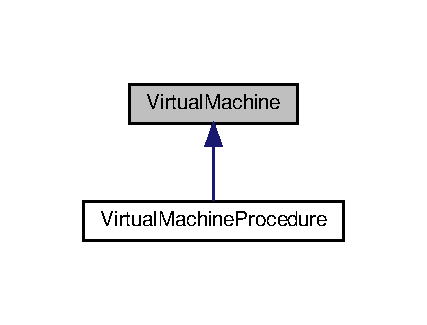
\includegraphics[width=205pt]{classVirtualMachine__inherit__graph}
\end{center}
\end{figure}


Collaboration diagram for Virtual\+Machine\+:\nopagebreak
\begin{figure}[H]
\begin{center}
\leavevmode
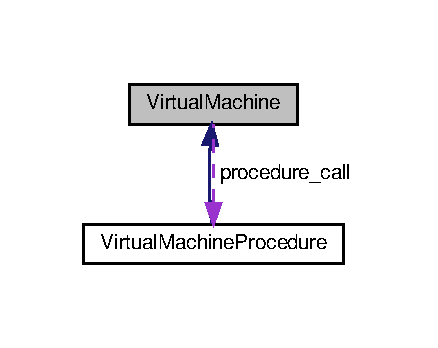
\includegraphics[width=210pt]{classVirtualMachine__coll__graph}
\end{center}
\end{figure}
\subsection*{Public Member Functions}
\begin{DoxyCompactItemize}
\item 
\hyperlink{classVirtualMachine_a81dc06209be015ba53fd1ad93a3a5ef7}{Virtual\+Machine} (const string \&program, istream $\ast$in, ostream $\ast$out, size\+\_\+t size=30000, int $\ast$memory=nullptr)
\item 
void \hyperlink{classVirtualMachine_aa6de427678b13e4cb1900d33db279cbf}{do\+\_\+one\+\_\+iteration} (bool advance=true)
\item 
virtual void \hyperlink{classVirtualMachine_a85bd42167c75161f0dad72349214707c}{loop} ()
\item 
size\+\_\+t \hyperlink{classVirtualMachine_ace7438bc3a4fa6c0acedb8636a5354ab}{get\+\_\+size} ()
\item 
int \hyperlink{classVirtualMachine_a5d4cc0de286c14e8f02eb00d6cc8d3e4}{get\+\_\+current\+\_\+operator} ()
\item 
int \hyperlink{classVirtualMachine_ac93b4e3d667d479eab4193e38e59ec65}{get\+\_\+status} ()
\item 
int $\ast$ \hyperlink{classVirtualMachine_ab66b22be50763f52d2ff5666251df4d7}{get\+\_\+memory} ()
\item 
int $\ast$ \hyperlink{classVirtualMachine_a4a3c3c348eff0f3384ba96ad770886df}{get\+\_\+memory\+\_\+ptr} ()
\item 
void \hyperlink{classVirtualMachine_aca58b7d73d8594aa0c511459e997cdcc}{be\+\_\+verbose} ()
\item 
void \hyperlink{classVirtualMachine_af80080c053a7f4b6c9f53444a4ce2244}{stop\+\_\+verbose} ()
\item 
void \hyperlink{classVirtualMachine_a7461728411b1ef5889827be0fd3f47db}{be\+\_\+verbose\+\_\+procedure} ()
\item 
void \hyperlink{classVirtualMachine_a5eac3ead95ba1cb818c0634bd758cfc2}{stop\+\_\+verbose\+\_\+procedure} ()
\item 
virtual \hyperlink{classVirtualMachine_ab12bb31d1f511018a0a8e956efb72591}{operator string} ()
\item 
\mbox{\Hypertarget{classVirtualMachine_a971c4f5c3c04096e25e727642f672344}\label{classVirtualMachine_a971c4f5c3c04096e25e727642f672344}} 
ostream \& {\bfseries operator$<$$<$} (ostream \&o)
\end{DoxyCompactItemize}
\subsection*{Protected Member Functions}
\begin{DoxyCompactItemize}
\item 
\mbox{\Hypertarget{classVirtualMachine_a00fd4c9a26c49fbbc44e20029e2a4b5a}\label{classVirtualMachine_a00fd4c9a26c49fbbc44e20029e2a4b5a}} 
void {\bfseries initialize\+\_\+anchor\+\_\+map} ()
\item 
\mbox{\Hypertarget{classVirtualMachine_a831099c5103644994409bfb05158fcfa}\label{classVirtualMachine_a831099c5103644994409bfb05158fcfa}} 
void {\bfseries ptr\+\_\+incr} ()
\item 
\mbox{\Hypertarget{classVirtualMachine_a3337809db225885a4a767ab9a4e827be}\label{classVirtualMachine_a3337809db225885a4a767ab9a4e827be}} 
void {\bfseries ptr\+\_\+dincr} ()
\item 
\mbox{\Hypertarget{classVirtualMachine_a39405fbc2b37978eb0caaf1cf7822c81}\label{classVirtualMachine_a39405fbc2b37978eb0caaf1cf7822c81}} 
void {\bfseries val\+\_\+incr} ()
\item 
\mbox{\Hypertarget{classVirtualMachine_a4ececf3e5748ecc7dd08ba0bcf16708b}\label{classVirtualMachine_a4ececf3e5748ecc7dd08ba0bcf16708b}} 
void {\bfseries val\+\_\+dincr} ()
\item 
\mbox{\Hypertarget{classVirtualMachine_ac77e5ad35f59aaac531a50fb050088be}\label{classVirtualMachine_ac77e5ad35f59aaac531a50fb050088be}} 
virtual void {\bfseries val\+\_\+out} ()
\item 
\mbox{\Hypertarget{classVirtualMachine_a4c4d2727fab7e225f1bbc4bcf179334a}\label{classVirtualMachine_a4c4d2727fab7e225f1bbc4bcf179334a}} 
void {\bfseries char\+\_\+out} ()
\item 
\mbox{\Hypertarget{classVirtualMachine_ae48e3658153af738a27a7a1b51dfa824}\label{classVirtualMachine_ae48e3658153af738a27a7a1b51dfa824}} 
virtual void {\bfseries val\+\_\+in} ()
\item 
\mbox{\Hypertarget{classVirtualMachine_a10bacaf18d480f8dd6b3965b1e5bdf54}\label{classVirtualMachine_a10bacaf18d480f8dd6b3965b1e5bdf54}} 
void {\bfseries handle\+\_\+bracket} ()
\item 
\mbox{\Hypertarget{classVirtualMachine_af90bdd5633e01c2f3bc29bd5899dc059}\label{classVirtualMachine_af90bdd5633e01c2f3bc29bd5899dc059}} 
void {\bfseries go\+\_\+to\+\_\+cond} ()
\item 
\mbox{\Hypertarget{classVirtualMachine_a8cef064caf26cd37e8f251fe872e0b3d}\label{classVirtualMachine_a8cef064caf26cd37e8f251fe872e0b3d}} 
void {\bfseries go\+\_\+to} ()
\item 
\mbox{\Hypertarget{classVirtualMachine_af94090fc2b0e8551f1c95cafb3a9d8bc}\label{classVirtualMachine_af94090fc2b0e8551f1c95cafb3a9d8bc}} 
void {\bfseries go\+\_\+to\+\_\+anchor} (int anchor)
\item 
\mbox{\Hypertarget{classVirtualMachine_ab586084441d2ca727d5b9f53f7ebd477}\label{classVirtualMachine_ab586084441d2ca727d5b9f53f7ebd477}} 
void {\bfseries exit\+\_\+goto} ()
\item 
\mbox{\Hypertarget{classVirtualMachine_a7f30065e78fd873c790d74af160c869d}\label{classVirtualMachine_a7f30065e78fd873c790d74af160c869d}} 
void {\bfseries ptr\+\_\+jump} ()
\item 
\mbox{\Hypertarget{classVirtualMachine_ad73ecf890b9d849c6310f77057d4b87b}\label{classVirtualMachine_ad73ecf890b9d849c6310f77057d4b87b}} 
void {\bfseries ptr\+\_\+reset} ()
\item 
\mbox{\Hypertarget{classVirtualMachine_a71799daec78aaa1e167882d8f3e8af18}\label{classVirtualMachine_a71799daec78aaa1e167882d8f3e8af18}} 
void {\bfseries val\+\_\+reset} ()
\item 
\mbox{\Hypertarget{classVirtualMachine_a17be3c7ea289013289f241f0031910ed}\label{classVirtualMachine_a17be3c7ea289013289f241f0031910ed}} 
void {\bfseries do\+\_\+n\+\_\+time} ()
\item 
\mbox{\Hypertarget{classVirtualMachine_abf6322c8307ff0b852a06006420e5195}\label{classVirtualMachine_abf6322c8307ff0b852a06006420e5195}} 
void {\bfseries call\+\_\+procedure} ()
\item 
\mbox{\Hypertarget{classVirtualMachine_aa3ee3502f78362500f80bc0080f3dd9c}\label{classVirtualMachine_aa3ee3502f78362500f80bc0080f3dd9c}} 
string {\bfseries file\+\_\+to\+\_\+string} (string filename)
\item 
\mbox{\Hypertarget{classVirtualMachine_a8942cd39f71a15aa88377900971e5580}\label{classVirtualMachine_a8942cd39f71a15aa88377900971e5580}} 
void {\bfseries loop\+\_\+procedure} ()
\item 
\mbox{\Hypertarget{classVirtualMachine_a1aaf05a7527d81bea2590e41a4c8cf7a}\label{classVirtualMachine_a1aaf05a7527d81bea2590e41a4c8cf7a}} 
void {\bfseries terminate\+\_\+procedure} ()
\item 
\mbox{\Hypertarget{classVirtualMachine_ab75d29be266f5be1f20de19ed9f62ef4}\label{classVirtualMachine_ab75d29be266f5be1f20de19ed9f62ef4}} 
virtual void {\bfseries error_handler} (int code)
\item 
\mbox{\Hypertarget{classVirtualMachine_a415a13dbb9c3cf07616d36e8692c2933}\label{classVirtualMachine_a415a13dbb9c3cf07616d36e8692c2933}} 
int {\bfseries extract\+\_\+number\+\_\+from\+\_\+program} (unsigned int start\+\_\+address, size\+\_\+t $\ast$t=nullptr)
\item 
\mbox{\Hypertarget{classVirtualMachine_a82d86e8e22643a11278cd9f05b5addff}\label{classVirtualMachine_a82d86e8e22643a11278cd9f05b5addff}} 
virtual void {\bfseries message} (const string \&message)
\item 
\mbox{\Hypertarget{classVirtualMachine_a9b4a8d2a6b18f98f3bd00390bed78a79}\label{classVirtualMachine_a9b4a8d2a6b18f98f3bd00390bed78a79}} 
virtual string {\bfseries memory\+\_\+to\+\_\+string} ()
\item 
\mbox{\Hypertarget{classVirtualMachine_a13c1e801e7d9a8afae6c92902044cc45}\label{classVirtualMachine_a13c1e801e7d9a8afae6c92902044cc45}} 
virtual string {\bfseries program\+\_\+to\+\_\+string} ()
\end{DoxyCompactItemize}
\subsection*{Protected Attributes}
\begin{DoxyCompactItemize}
\item 
\mbox{\Hypertarget{classVirtualMachine_a4d60f4b532942602eee8492ab0d21afc}\label{classVirtualMachine_a4d60f4b532942602eee8492ab0d21afc}} 
string {\bfseries program}
\item 
\mbox{\Hypertarget{classVirtualMachine_a91504e81123c4799eb86397567adf124}\label{classVirtualMachine_a91504e81123c4799eb86397567adf124}} 
istream $\ast$ {\bfseries in}
\item 
\mbox{\Hypertarget{classVirtualMachine_a2536e46cc553233a55b5ce37174b805e}\label{classVirtualMachine_a2536e46cc553233a55b5ce37174b805e}} 
ostream $\ast$ {\bfseries out}
\item 
\mbox{\Hypertarget{classVirtualMachine_ac34063086f2ac1fcf0948b047e21d7d3}\label{classVirtualMachine_ac34063086f2ac1fcf0948b047e21d7d3}} 
size\+\_\+t {\bfseries size}
\item 
\mbox{\Hypertarget{classVirtualMachine_a181524e58d377d458ce08789392edd05}\label{classVirtualMachine_a181524e58d377d458ce08789392edd05}} 
int $\ast$ {\bfseries memory}
\item 
\mbox{\Hypertarget{classVirtualMachine_a70e4bcf4a8dc15f1bd2623f174911949}\label{classVirtualMachine_a70e4bcf4a8dc15f1bd2623f174911949}} 
int $\ast$ {\bfseries memory\+\_\+ptr}
\item 
\mbox{\Hypertarget{classVirtualMachine_aa1fe839b3c60ed06f08d25234a942fec}\label{classVirtualMachine_aa1fe839b3c60ed06f08d25234a942fec}} 
unsigned int {\bfseries current\+\_\+operator}
\item 
\mbox{\Hypertarget{classVirtualMachine_aaca3982311ac4bb0fcdc245c917cb0c9}\label{classVirtualMachine_aaca3982311ac4bb0fcdc245c917cb0c9}} 
int {\bfseries status}
\item 
\mbox{\Hypertarget{classVirtualMachine_a6f03a3c1e97c82b919d40216dada8a62}\label{classVirtualMachine_a6f03a3c1e97c82b919d40216dada8a62}} 
bool {\bfseries verbose}
\item 
\mbox{\Hypertarget{classVirtualMachine_a32813e2f6f744d057ff3fb3247263ce6}\label{classVirtualMachine_a32813e2f6f744d057ff3fb3247263ce6}} 
bool {\bfseries verbose\+\_\+procedure}
\item 
\mbox{\Hypertarget{classVirtualMachine_a79c1eaa2d795cb60a3046f5602e73b55}\label{classVirtualMachine_a79c1eaa2d795cb60a3046f5602e73b55}} 
map$<$ unsigned int, unsigned int $>$ {\bfseries anchor\+\_\+map}
\item 
\mbox{\Hypertarget{classVirtualMachine_a4dcdbb9cd441a4f356212cf1dcabab9c}\label{classVirtualMachine_a4dcdbb9cd441a4f356212cf1dcabab9c}} 
int {\bfseries depth}
\item 
\mbox{\Hypertarget{classVirtualMachine_a7ed46115fe6a39029de0674aa4fa69fd}\label{classVirtualMachine_a7ed46115fe6a39029de0674aa4fa69fd}} 
\hyperlink{classVirtualMachineProcedure}{Virtual\+Machine\+Procedure} $\ast$ {\bfseries procedure\+\_\+call}
\end{DoxyCompactItemize}


\subsection{Detailed Description}
This is the language interpreter class 

\subsection{Constructor \& Destructor Documentation}
\mbox{\Hypertarget{classVirtualMachine_a81dc06209be015ba53fd1ad93a3a5ef7}\label{classVirtualMachine_a81dc06209be015ba53fd1ad93a3a5ef7}} 
\index{Virtual\+Machine@{Virtual\+Machine}!Virtual\+Machine@{Virtual\+Machine}}
\index{Virtual\+Machine@{Virtual\+Machine}!Virtual\+Machine@{Virtual\+Machine}}
\subsubsection{\texorpdfstring{Virtual\+Machine()}{VirtualMachine()}}
{\footnotesize\ttfamily Virtual\+Machine\+::\+Virtual\+Machine (\begin{DoxyParamCaption}\item[{const string \&}]{program,  }\item[{istream $\ast$}]{in,  }\item[{ostream $\ast$}]{out,  }\item[{size\+\_\+t}]{size = {\ttfamily 30000},  }\item[{int $\ast$}]{memory = {\ttfamily nullptr} }\end{DoxyParamCaption})}

Constructor that initializes all the fields 
\begin{DoxyParams}{Parameters}
{\em program} & The code to be executed \\
\hline
{\em in} & The input stream \\
\hline
{\em out} & The output stream \\
\hline
{\em size} & The size of the memory. If the program starts with a number, this will be ignored \\
\hline
{\em memory} & The memory to be used by the machine. Allocated automatically if not specified. \\
\hline
\end{DoxyParams}


\subsection{Member Function Documentation}
\mbox{\Hypertarget{classVirtualMachine_aca58b7d73d8594aa0c511459e997cdcc}\label{classVirtualMachine_aca58b7d73d8594aa0c511459e997cdcc}} 
\index{Virtual\+Machine@{Virtual\+Machine}!be\+\_\+verbose@{be\+\_\+verbose}}
\index{be\+\_\+verbose@{be\+\_\+verbose}!Virtual\+Machine@{Virtual\+Machine}}
\subsubsection{\texorpdfstring{be\+\_\+verbose()}{be\_verbose()}}
{\footnotesize\ttfamily void Virtual\+Machine\+::be\+\_\+verbose (\begin{DoxyParamCaption}{ }\end{DoxyParamCaption})}

Makes the VM verbose. \mbox{\Hypertarget{classVirtualMachine_a7461728411b1ef5889827be0fd3f47db}\label{classVirtualMachine_a7461728411b1ef5889827be0fd3f47db}} 
\index{Virtual\+Machine@{Virtual\+Machine}!be\+\_\+verbose\+\_\+procedure@{be\+\_\+verbose\+\_\+procedure}}
\index{be\+\_\+verbose\+\_\+procedure@{be\+\_\+verbose\+\_\+procedure}!Virtual\+Machine@{Virtual\+Machine}}
\subsubsection{\texorpdfstring{be\+\_\+verbose\+\_\+procedure()}{be\_verbose\_procedure()}}
{\footnotesize\ttfamily void Virtual\+Machine\+::be\+\_\+verbose\+\_\+procedure (\begin{DoxyParamCaption}{ }\end{DoxyParamCaption})}

Make the VM and its procedures verbose. \mbox{\Hypertarget{classVirtualMachine_aa6de427678b13e4cb1900d33db279cbf}\label{classVirtualMachine_aa6de427678b13e4cb1900d33db279cbf}} 
\index{Virtual\+Machine@{Virtual\+Machine}!do\+\_\+one\+\_\+iteration@{do\+\_\+one\+\_\+iteration}}
\index{do\+\_\+one\+\_\+iteration@{do\+\_\+one\+\_\+iteration}!Virtual\+Machine@{Virtual\+Machine}}
\subsubsection{\texorpdfstring{do\+\_\+one\+\_\+iteration()}{do\_one\_iteration()}}
{\footnotesize\ttfamily void Virtual\+Machine\+::do\+\_\+one\+\_\+iteration (\begin{DoxyParamCaption}\item[{bool}]{advance = {\ttfamily true} }\end{DoxyParamCaption})}

This do one iteration of the execution 
\begin{DoxyParams}{Parameters}
{\em advance} & This bool is here to tell the VM if it should advance in the program or redo the same operator next time. \\
\hline
\end{DoxyParams}
\mbox{\Hypertarget{classVirtualMachine_a5d4cc0de286c14e8f02eb00d6cc8d3e4}\label{classVirtualMachine_a5d4cc0de286c14e8f02eb00d6cc8d3e4}} 
\index{Virtual\+Machine@{Virtual\+Machine}!get\+\_\+current\+\_\+operator@{get\+\_\+current\+\_\+operator}}
\index{get\+\_\+current\+\_\+operator@{get\+\_\+current\+\_\+operator}!Virtual\+Machine@{Virtual\+Machine}}
\subsubsection{\texorpdfstring{get\+\_\+current\+\_\+operator()}{get\_current\_operator()}}
{\footnotesize\ttfamily int Virtual\+Machine\+::get\+\_\+current\+\_\+operator (\begin{DoxyParamCaption}{ }\end{DoxyParamCaption})}

Getter for member current\+\_\+operator \begin{DoxyReturn}{Returns}
current\+\_\+operator 
\end{DoxyReturn}
\mbox{\Hypertarget{classVirtualMachine_ab66b22be50763f52d2ff5666251df4d7}\label{classVirtualMachine_ab66b22be50763f52d2ff5666251df4d7}} 
\index{Virtual\+Machine@{Virtual\+Machine}!get\+\_\+memory@{get\+\_\+memory}}
\index{get\+\_\+memory@{get\+\_\+memory}!Virtual\+Machine@{Virtual\+Machine}}
\subsubsection{\texorpdfstring{get\+\_\+memory()}{get\_memory()}}
{\footnotesize\ttfamily int $\ast$ Virtual\+Machine\+::get\+\_\+memory (\begin{DoxyParamCaption}{ }\end{DoxyParamCaption})}

Getter for member memory \begin{DoxyReturn}{Returns}
memory 
\end{DoxyReturn}
\mbox{\Hypertarget{classVirtualMachine_a4a3c3c348eff0f3384ba96ad770886df}\label{classVirtualMachine_a4a3c3c348eff0f3384ba96ad770886df}} 
\index{Virtual\+Machine@{Virtual\+Machine}!get\+\_\+memory\+\_\+ptr@{get\+\_\+memory\+\_\+ptr}}
\index{get\+\_\+memory\+\_\+ptr@{get\+\_\+memory\+\_\+ptr}!Virtual\+Machine@{Virtual\+Machine}}
\subsubsection{\texorpdfstring{get\+\_\+memory\+\_\+ptr()}{get\_memory\_ptr()}}
{\footnotesize\ttfamily int $\ast$ Virtual\+Machine\+::get\+\_\+memory\+\_\+ptr (\begin{DoxyParamCaption}{ }\end{DoxyParamCaption})}

Getter for member memory\+\_\+ptr \begin{DoxyReturn}{Returns}
memory\+\_\+ptr 
\end{DoxyReturn}
\mbox{\Hypertarget{classVirtualMachine_ace7438bc3a4fa6c0acedb8636a5354ab}\label{classVirtualMachine_ace7438bc3a4fa6c0acedb8636a5354ab}} 
\index{Virtual\+Machine@{Virtual\+Machine}!get\+\_\+size@{get\+\_\+size}}
\index{get\+\_\+size@{get\+\_\+size}!Virtual\+Machine@{Virtual\+Machine}}
\subsubsection{\texorpdfstring{get\+\_\+size()}{get\_size()}}
{\footnotesize\ttfamily size\+\_\+t Virtual\+Machine\+::get\+\_\+size (\begin{DoxyParamCaption}{ }\end{DoxyParamCaption})}

Getter for member size \begin{DoxyReturn}{Returns}
size 
\end{DoxyReturn}
\mbox{\Hypertarget{classVirtualMachine_ac93b4e3d667d479eab4193e38e59ec65}\label{classVirtualMachine_ac93b4e3d667d479eab4193e38e59ec65}} 
\index{Virtual\+Machine@{Virtual\+Machine}!get\+\_\+status@{get\+\_\+status}}
\index{get\+\_\+status@{get\+\_\+status}!Virtual\+Machine@{Virtual\+Machine}}
\subsubsection{\texorpdfstring{get\+\_\+status()}{get\_status()}}
{\footnotesize\ttfamily int Virtual\+Machine\+::get\+\_\+status (\begin{DoxyParamCaption}{ }\end{DoxyParamCaption})}

Getter for member status \begin{DoxyReturn}{Returns}
status 
\end{DoxyReturn}
\mbox{\Hypertarget{classVirtualMachine_a85bd42167c75161f0dad72349214707c}\label{classVirtualMachine_a85bd42167c75161f0dad72349214707c}} 
\index{Virtual\+Machine@{Virtual\+Machine}!loop@{loop}}
\index{loop@{loop}!Virtual\+Machine@{Virtual\+Machine}}
\subsubsection{\texorpdfstring{loop()}{loop()}}
{\footnotesize\ttfamily void Virtual\+Machine\+::loop (\begin{DoxyParamCaption}{ }\end{DoxyParamCaption})\hspace{0.3cm}{\ttfamily [virtual]}}

This execute the program until it halts. \mbox{\Hypertarget{classVirtualMachine_ab12bb31d1f511018a0a8e956efb72591}\label{classVirtualMachine_ab12bb31d1f511018a0a8e956efb72591}} 
\index{Virtual\+Machine@{Virtual\+Machine}!operator string@{operator string}}
\index{operator string@{operator string}!Virtual\+Machine@{Virtual\+Machine}}
\subsubsection{\texorpdfstring{operator string()}{operator string()}}
{\footnotesize\ttfamily Virtual\+Machine\+::operator string (\begin{DoxyParamCaption}{ }\end{DoxyParamCaption})\hspace{0.3cm}{\ttfamily [explicit]}, {\ttfamily [virtual]}}

Convert the VM\textquotesingle{}s current state into a string. \begin{DoxyReturn}{Returns}
The VM\textquotesingle{}s string representation 
\end{DoxyReturn}


Reimplemented in \hyperlink{classVirtualMachineProcedure_aea6310148a612586e5fd9e30650decb6}{Virtual\+Machine\+Procedure}.

\mbox{\Hypertarget{classVirtualMachine_af80080c053a7f4b6c9f53444a4ce2244}\label{classVirtualMachine_af80080c053a7f4b6c9f53444a4ce2244}} 
\index{Virtual\+Machine@{Virtual\+Machine}!stop\+\_\+verbose@{stop\+\_\+verbose}}
\index{stop\+\_\+verbose@{stop\+\_\+verbose}!Virtual\+Machine@{Virtual\+Machine}}
\subsubsection{\texorpdfstring{stop\+\_\+verbose()}{stop\_verbose()}}
{\footnotesize\ttfamily void Virtual\+Machine\+::stop\+\_\+verbose (\begin{DoxyParamCaption}{ }\end{DoxyParamCaption})}

Makes the VM silent. \mbox{\Hypertarget{classVirtualMachine_a5eac3ead95ba1cb818c0634bd758cfc2}\label{classVirtualMachine_a5eac3ead95ba1cb818c0634bd758cfc2}} 
\index{Virtual\+Machine@{Virtual\+Machine}!stop\+\_\+verbose\+\_\+procedure@{stop\+\_\+verbose\+\_\+procedure}}
\index{stop\+\_\+verbose\+\_\+procedure@{stop\+\_\+verbose\+\_\+procedure}!Virtual\+Machine@{Virtual\+Machine}}
\subsubsection{\texorpdfstring{stop\+\_\+verbose\+\_\+procedure()}{stop\_verbose\_procedure()}}
{\footnotesize\ttfamily void Virtual\+Machine\+::stop\+\_\+verbose\+\_\+procedure (\begin{DoxyParamCaption}{ }\end{DoxyParamCaption})}

Make the VM\textquotesingle{}s procedures silent. 

The documentation for this class was generated from the following files\+:\begin{DoxyCompactItemize}
\item 
/home/emile/etudes/\+L\+I\+F\+A\+P4/\+A\+Stressful\+Machine/src/Virtual\+Machine.\+h\item 
/home/emile/etudes/\+L\+I\+F\+A\+P4/\+A\+Stressful\+Machine/src/Virtual\+Machine.\+cpp\end{DoxyCompactItemize}

\hypertarget{classVirtualMachineProcedure}{}\section{Virtual\+Machine\+Procedure Class Reference}
\label{classVirtualMachineProcedure}\index{Virtual\+Machine\+Procedure@{Virtual\+Machine\+Procedure}}


{\ttfamily \#include $<$Virtual\+Machine\+Procedure.\+h$>$}



Inheritance diagram for Virtual\+Machine\+Procedure\+:\nopagebreak
\begin{figure}[H]
\begin{center}
\leavevmode
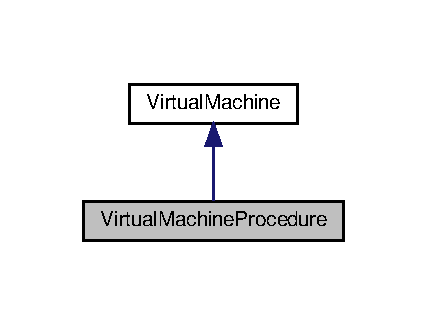
\includegraphics[width=205pt]{classVirtualMachineProcedure__inherit__graph}
\end{center}
\end{figure}


Collaboration diagram for Virtual\+Machine\+Procedure\+:\nopagebreak
\begin{figure}[H]
\begin{center}
\leavevmode
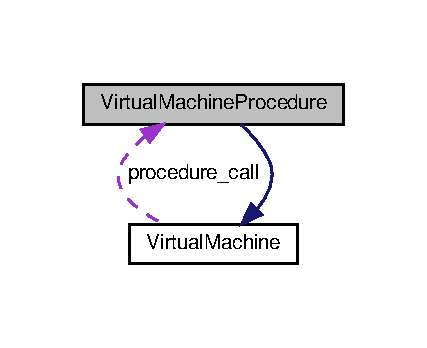
\includegraphics[width=205pt]{classVirtualMachineProcedure__coll__graph}
\end{center}
\end{figure}
\subsection*{Public Member Functions}
\begin{DoxyCompactItemize}
\item 
\hyperlink{classVirtualMachineProcedure_a3db90b62f4165b9d334134c361ebdc30}{Virtual\+Machine\+Procedure} (const string \&program, istream $\ast$in, ostream $\ast$out, int depth, size\+\_\+t size=30000, int $\ast$memory=nullptr)
\item 
int \hyperlink{classVirtualMachineProcedure_a608e8e83938e5b29a11c5b26671d3654}{get\+\_\+output} ()
\item 
\mbox{\Hypertarget{classVirtualMachineProcedure_a71d8552422569e57903212d51f38c6ee}\label{classVirtualMachineProcedure_a71d8552422569e57903212d51f38c6ee}} 
void {\bfseries input} (int inpt)
\item 
\hyperlink{classVirtualMachineProcedure_aea6310148a612586e5fd9e30650decb6}{operator string} () override
\end{DoxyCompactItemize}
\subsection*{Public Attributes}
\begin{DoxyCompactItemize}
\item 
\mbox{\Hypertarget{classVirtualMachineProcedure_a95e6694d96087741291ca2ecf3009b97}\label{classVirtualMachineProcedure_a95e6694d96087741291ca2ecf3009b97}} 
int {\bfseries depth}
\end{DoxyCompactItemize}
\subsection*{Protected Member Functions}
\begin{DoxyCompactItemize}
\item 
\mbox{\Hypertarget{classVirtualMachineProcedure_aa6f5e4488e0b6a09da5d27fa2cf8e156}\label{classVirtualMachineProcedure_aa6f5e4488e0b6a09da5d27fa2cf8e156}} 
void {\bfseries val\+\_\+out} () override
\item 
\mbox{\Hypertarget{classVirtualMachineProcedure_a868e4133bc5fcfb969de2d3d6f6008fe}\label{classVirtualMachineProcedure_a868e4133bc5fcfb969de2d3d6f6008fe}} 
void {\bfseries val\+\_\+in} () override
\item 
\mbox{\Hypertarget{classVirtualMachineProcedure_a20aa263ac34a0e01d5a11cbfe919cb4f}\label{classVirtualMachineProcedure_a20aa263ac34a0e01d5a11cbfe919cb4f}} 
void {\bfseries error} (int code) override
\item 
\mbox{\Hypertarget{classVirtualMachineProcedure_a755d40765bb540503a9bea5ffd091a46}\label{classVirtualMachineProcedure_a755d40765bb540503a9bea5ffd091a46}} 
void {\bfseries message} (const string \&message) override
\end{DoxyCompactItemize}
\subsection*{Protected Attributes}
\begin{DoxyCompactItemize}
\item 
\mbox{\Hypertarget{classVirtualMachineProcedure_a0d82fcd19a990a5ad6d0bc51d25b5977}\label{classVirtualMachineProcedure_a0d82fcd19a990a5ad6d0bc51d25b5977}} 
int {\bfseries output}
\end{DoxyCompactItemize}


\subsection{Detailed Description}
This class is used by \hyperlink{classVirtualMachine}{Virtual\+Machine} to perform procedure calls. It is only the input and output and the verbose/error_handler printing that are changed.

\subsection{Constructor \& Destructor Documentation}
\mbox{\Hypertarget{classVirtualMachineProcedure_a3db90b62f4165b9d334134c361ebdc30}\label{classVirtualMachineProcedure_a3db90b62f4165b9d334134c361ebdc30}} 
\index{Virtual\+Machine\+Procedure@{Virtual\+Machine\+Procedure}!Virtual\+Machine\+Procedure@{Virtual\+Machine\+Procedure}}
\index{Virtual\+Machine\+Procedure@{Virtual\+Machine\+Procedure}!Virtual\+Machine\+Procedure@{Virtual\+Machine\+Procedure}}
\subsubsection{\texorpdfstring{Virtual\+Machine\+Procedure()}{VirtualMachineProcedure()}}
{\footnotesize\ttfamily Virtual\+Machine\+Procedure\+::\+Virtual\+Machine\+Procedure (\begin{DoxyParamCaption}\item[{const string \&}]{program,  }\item[{istream $\ast$}]{in,  }\item[{ostream $\ast$}]{out,  }\item[{int}]{depth,  }\item[{size\+\_\+t}]{size = {\ttfamily 30000},  }\item[{int $\ast$}]{memory = {\ttfamily nullptr} }\end{DoxyParamCaption})}

This call the \hyperlink{classVirtualMachine}{Virtual\+Machine} constructor as a delegate constructor and initialize the new fields. 
\begin{DoxyParams}{Parameters}
{\em program} & \\
\hline
{\em in} & \\
\hline
{\em out} & \\
\hline
{\em depth} & The recursive depth of the procedure. \\
\hline
{\em size} & \\
\hline
{\em memory} & \\
\hline
\end{DoxyParams}


\subsection{Member Function Documentation}
\mbox{\Hypertarget{classVirtualMachineProcedure_a608e8e83938e5b29a11c5b26671d3654}\label{classVirtualMachineProcedure_a608e8e83938e5b29a11c5b26671d3654}} 
\index{Virtual\+Machine\+Procedure@{Virtual\+Machine\+Procedure}!get\+\_\+output@{get\+\_\+output}}
\index{get\+\_\+output@{get\+\_\+output}!Virtual\+Machine\+Procedure@{Virtual\+Machine\+Procedure}}
\subsubsection{\texorpdfstring{get\+\_\+output()}{get\_output()}}
{\footnotesize\ttfamily int Virtual\+Machine\+Procedure\+::get\+\_\+output (\begin{DoxyParamCaption}{ }\end{DoxyParamCaption})}

This should be used to access the output of the procedure. \begin{DoxyReturn}{Returns}
The output of the procedure 
\end{DoxyReturn}
\mbox{\Hypertarget{classVirtualMachineProcedure_aea6310148a612586e5fd9e30650decb6}\label{classVirtualMachineProcedure_aea6310148a612586e5fd9e30650decb6}} 
\index{Virtual\+Machine\+Procedure@{Virtual\+Machine\+Procedure}!operator string@{operator string}}
\index{operator string@{operator string}!Virtual\+Machine\+Procedure@{Virtual\+Machine\+Procedure}}
\subsubsection{\texorpdfstring{operator string()}{operator string()}}
{\footnotesize\ttfamily Virtual\+Machine\+Procedure\+::operator string (\begin{DoxyParamCaption}{ }\end{DoxyParamCaption})\hspace{0.3cm}{\ttfamily [explicit]}, {\ttfamily [override]}, {\ttfamily [virtual]}}

Convert the VM\textquotesingle{}s current state into a string. \begin{DoxyReturn}{Returns}
The VM\textquotesingle{}s string representation 
\end{DoxyReturn}


Reimplemented from \hyperlink{classVirtualMachine_ab12bb31d1f511018a0a8e956efb72591}{Virtual\+Machine}.



The documentation for this class was generated from the following files\+:\begin{DoxyCompactItemize}
\item 
/home/emile/etudes/\+L\+I\+F\+A\+P4/\+A\+Stressful\+Machine/src/Virtual\+Machine\+Procedure.\+h\item 
/home/emile/etudes/\+L\+I\+F\+A\+P4/\+A\+Stressful\+Machine/src/Virtual\+Machine\+Procedure.\+cpp\end{DoxyCompactItemize}

%--- End generated contents ---

% Index
\backmatter
\newpage
\phantomsection
\clearemptydoublepage
\addcontentsline{toc}{chapter}{Index}
\printindex

\end{document}
